%!TEX root = ../../../../thesis.tex
\section{Natural computing with P. Polycephalum}

	It can be argued that a necessary precursor to \P being discovered as a suitable substrate for natural computing consist of a series of break-through experiments of Nakagaki et al. that changed our perception of the unassuming organisms that are slime molds.
	
	The first of which was introduced in the year 2000. In the so-called ``maze experiment'' the plasmodium of \P is introduced to a maze, see \Fref{fig:maze:initial}~\cite{nakagaki2000intelligence}. After the plasmodium has spread evenly across the entire maze, two food sources are introduced at two specific points in the maze, see \Fref{fig:maze:intermediate}. The organism forms veins while slowly retracting from areas of the maze that do not intersect with any path connecting the two food sources. This process continues until the plasmodium takes the shape of one single thick vein connecting the food sources. In repeated experiments, it was shown that the organism occupies precisely the shortest path ($\alpha_1 + \beta_1$) in most of the cases. This demonstrates the organisms remarkable ability of iteratively improving the connection between the two food sources.
	In this context an improvement is achieved if veins become either shorter or wider in diameter. Since nutrient transport is subject to hydrodynamic forces, shorter and wider tubes entail less resistance to fluid flow~\cite{kamiya1959motive}.

	One may interpret the maze as a graph with edge weights equal to the lengths of the associated maze segments and the food sources as two distinct nodes $N_1$ and $N_2$, see~\Fref{fig:maze:abstraction}. Thus the slime mold \Pp can be seen to demonstrate a solution to the $s-t$ shortest path problem with $s=N_1$ and $t=N_2$.

	\begin{figure}
		\centering
		\subfloat[Maze experiment - Initial state][]{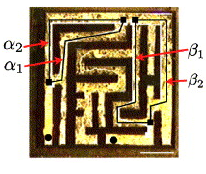
\includegraphics[width=0.45\linewidth,keepaspectratio]{maze/maze_experiment_1.png}\label{fig:maze:initial}}
		\subfloat[Maze experiment - Intermediate state][]{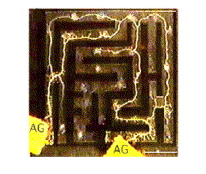
\includegraphics[width=0.45\linewidth,keepaspectratio]{maze/maze_experiment_2.png}\label{fig:maze:intermediate}}
		\newline
		\subfloat[Maze experiment - Final state][]{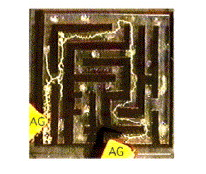
\includegraphics[width=0.45\linewidth,keepaspectratio]{maze/maze_experiment_3.png}\label{fig:maze:final}}
		\subfloat[Maze experiment - Graph abstraction][]{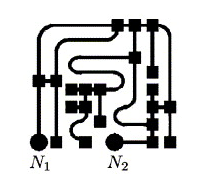
\includegraphics[width=0.45\linewidth,keepaspectratio]{maze/maze_experiment_4.png}\label{fig:maze:abstraction}}
		
		\caption[Classic maze experiment with \P]{ a) The plasmodium of 
		\P is evenly spread across a maze. Filled black circles denote two specific points in the maze. Arrows indicate segments of possible paths between them. b) Two food sources (AG) are introduced at the specific points. After a while the plasmodium retreats from areas of the maze that do not intersect with a path connecting the food sources. c) The plasmodium settles on the shortest path between the two food sources. d) The maze can be interpreted as an abstract graph with two distinct nodes $N_1$ and $N_2$ corresponding to the food sources. The scale bars denote 1 cm. Reprinted from~\cite{Tero2007553}.}
		\label{fig:maze}
	\end{figure}

	In 2004 \P was presented with three or more food sources arranged in a regular pattern~\cite{nakagaki2004obtaining}. In repeated experiments the organism was found to connect the food sources in patterns that frequently resemble well known structures such as minimum spanning trees and minimum steiner trees. The experimenters reported two empirical observations that seem to play a key role in the formation of \P networks: First open-ended or dead-end veins are likely to disappear as time goes by. And second, when more than one vein connects the same pair of food sources, all longer veins tend to disappear while the shortest vein is reinforced. 
	
	These observations have been explained on a physiological level in~\cite{Tero2006115}. The plasmodium of \P organizes itself through the formation of thick veins through which the protoplasm is driven as a result of periodic contractions of the veins themselves, \ie peristaltic pumping. The veins are formed if streaming of protoplasm persist in a given direction for a sufficiently long time~\cite{nakagaki2000interaction}. On a molecular scale Actomyosin fibers carried by the protoplasmic flow attach along the lengths of a vein resulting in tubular structures. The fast flowing protoplasm also causes shear stress, exerting a force which stretch-induces a regular orientation of the Actomyosin fibers. As a result, veins with a large flux manage to accumulate and orient additional Actomyosin fibers which over time leads to an increase in vein diameter. This in turn further reduces the resistance to flow because under the assumption that the fluid flow in the veins of \P is a Poiseuille flow, the theory of hydrodynamics dictates that it be proportional to the forth power of the vein diameter and inverse proportional to the vein length. It follows that veins that are carrying little flow either because they are long and/or thin or happen to be dead-end veins are likely to degenerate over time as experimentally observed above. At the same time, reinforcing thick and short veins ensures efficient fluid flow, which in turn enables effective circulation and transport of nutrients, nuclei and signaling molecules.

	These considerations became the basis of a concise model presented in 2006, which captures the behavior of the slime mold as demonstrated in the maze experiment and lead to the first natural computing approaches based on \P~\cite{Tero2006115}. The model can be formulated on a graph $G = (V,E)$, where the node set $V$ denotes the junction points of veins and the edge set $E$ denotes the veins themselves. Each node $u \in V$ has a hydrodynamic pressure associated with it denoted by $p_u(t)$. Each edge $e = (u,v) \in E$ has a length $L_e$ as well as a time-dependent flow through the vein $Q_e(t)$. Here it is assumed that the flow is a Poiseuille flow such that

	\begin{equation}
		Q_e(t) = \frac{\pi r_e(t)^4}{ 8 \eta} \frac{p_u(t)-p_v(t)}{L_e}
		\label{eq:flow_initial}
	\end{equation}
	
	holds. Here $r_e(t)$ is the diameter of an edge and $\eta$ refers to the viscosity of the protoplasmic fluid. Let $D_e(t) = \pi r(t)^4/ 8 \eta$. Then we can simplify \Fref{eq:flow_initial} to read

	\begin{equation}
		Q_e(t) = \frac{D_e(t)}{L_e} (p_i(t) - p_j(t)).
		\label{eq:flow}
	\end{equation}

	Let us choose two distinct nodes $s, t \in V$ representing the source and sink nodes in the graph. Using this definition we obtain an equation for each edge $e \in E$:

	\begin{equation}
		\sum_{e = (u,v) } Q_e(t) =
		\begin{cases}
		\quad 1 & \ \text{for} \ u=s, \\
		\quad -1 & \ \text{for} \ u=t, \\
		\quad 0 & \ \text{otherwise}.
		\end{cases}
		\label{eq:conservation_of_flow}
	\end{equation}
	Note that the l.h.s is chosen such that flow is conserved everywhere except at the source and the sink where flow is entering respectively leaving the graph. Thus one unit of flow is introduced to the system. \Fref{eq:conservation_of_flow} can be solved to obtain the values of the $Q(t)_e$ and the $p_u(t)$ simultaneously.

	Finally the time-dependence of $D(t)_e$ is choose such, that the positive feedback between $D(t)_e$ and $Q_e(t)$ is as described above. For each $e \in E$ the dimensionless equation for $D(t)_e$ reads

	\begin{equation}
		\frac{d}{dt} D_e(t) = f( Q(t)_e ) - D_e(t),
		\label{eq:evolution}
	\end{equation}
	which is called adaptation or \emph{evolution equation}. Here $f$ is a monotonically increasing continuous function such that $f(0) = 0$. \Fref{eq:evolution} is the key of the model which formalizes the experimental observations reported earlier. If at time $t$the flux through an edge is such that $f(Q_e(t)) < D_e(t)$ then $D_e(t)$ decreases which further reduces the flux through $e$. In this scenario an edge $e$ is degenerating. Likewise $f(Q_e(t)) > D_e(t)$ leads to an increase in $D_e(t)$ which further increases the flux. In this case $e$ is reinforced. Only ,$f(Q_e(t)) = D_e(t)$ enables a stationary state which leaves $D_e(t)$ and $Q_e(t)$ constant. 

	The model thus evolves the thickness of veins in \P according to \Fref{eq:evolution} relying on the values of $p_u(t)$ and $Q_e(t)$ which are governed by \Fref{eq:conservation_of_flow}. For suitable choices of $f(Q_e)$ this system can be discretized and solved numerically~\cite{Tero2006115}. For the graph depicted in~\Fref{fig:maze:abstraction} a stationary state was found where the $D_e(t)$ of all edges that do not belong to the shortest path between $s=N_1$ and $t=N_2$ vanished. At the same time $D_e(t)$ of the edge on the shortest path approached a constant. That is, just like the slime mold, the model has selected the shortest path in the graph connecting $s$ and $t$. 

	After this initial demonstration of the viability of \P as a medium for natural computing, computer scientists shortly thereafter started to analyze the model and its variants contributing a sequence of convergence proofs and complexity bounds. For suitable choices of $f(Q_e)$ convergence was proven for planar graphs at first~\cite{miyaji2007mathematical,miyaji2008physarum}, but shortly thereafter proofs were extended to general graphs for the original model and for variations thereof~\cite{Bonifaci2012121,bonifaci2013physarum,ito2011convergence,becchetti2013physarum}. The fact that the theoretical properties of the so-called \emph{Physarum solver} are rather well understood is a rarity amongst natural computing algorithms.

	

	The introduction of the physarum solver also triggered dedicated research efforts aimed at exploring the computational abilities of the slime mold further. The foraging behavior of \P was used in conjunction with several food sources to approximate structures such as minimum spanning trees, steiner trees or voronoi diagrams. More abstract experimental setups were constructed capable of exploiting the light-avoiding behavior of \P to solve small instances of the Travelling Salesman problem. 

	Efforts of harnessing these and other experimental demonstration in the form of models suitable for computation were pursued at the same time. One approach consists of modifying or repeatedly applyign the physarum solver in order to deal with several food sources. This has lead to algorithms that are capable of approximating the steiner minimum tree~\cite{6684158}, max flow, variations of the shortest path problem or physarum based network centrality.

	A second successful approach consists of modelling the behaviour of \P based on a particle swar model. In this model independent agents interact accroding to certain rules which lead to the emergence of global behaviour that resembles \P. This model is very flexible and was used to provide solutions to a range of problems including \todo[inline]{examples here \dots}.

	The disadvantages of these approaches are that the simulation of slime mold behavior in order to obtain a solution as often computationally expensive, even on small graphs. For these reason most algorithms are not competitive in terms of runtime when compared with existing algorithms. 

	However, the true merit of the natural computing lies in the fact that it pioneers a new paradigm of solving old problems. This in turn allows for a fresh approach leading to interesting new questions. While more efficient algorithms for a certain problem may already exist, it is not excluded that a natural computing approach based on \P or other media, yields a solution to some problem that has resisted efficient resolution up until now.

